
\subsection{Односторонние и двусторонние поверхности}
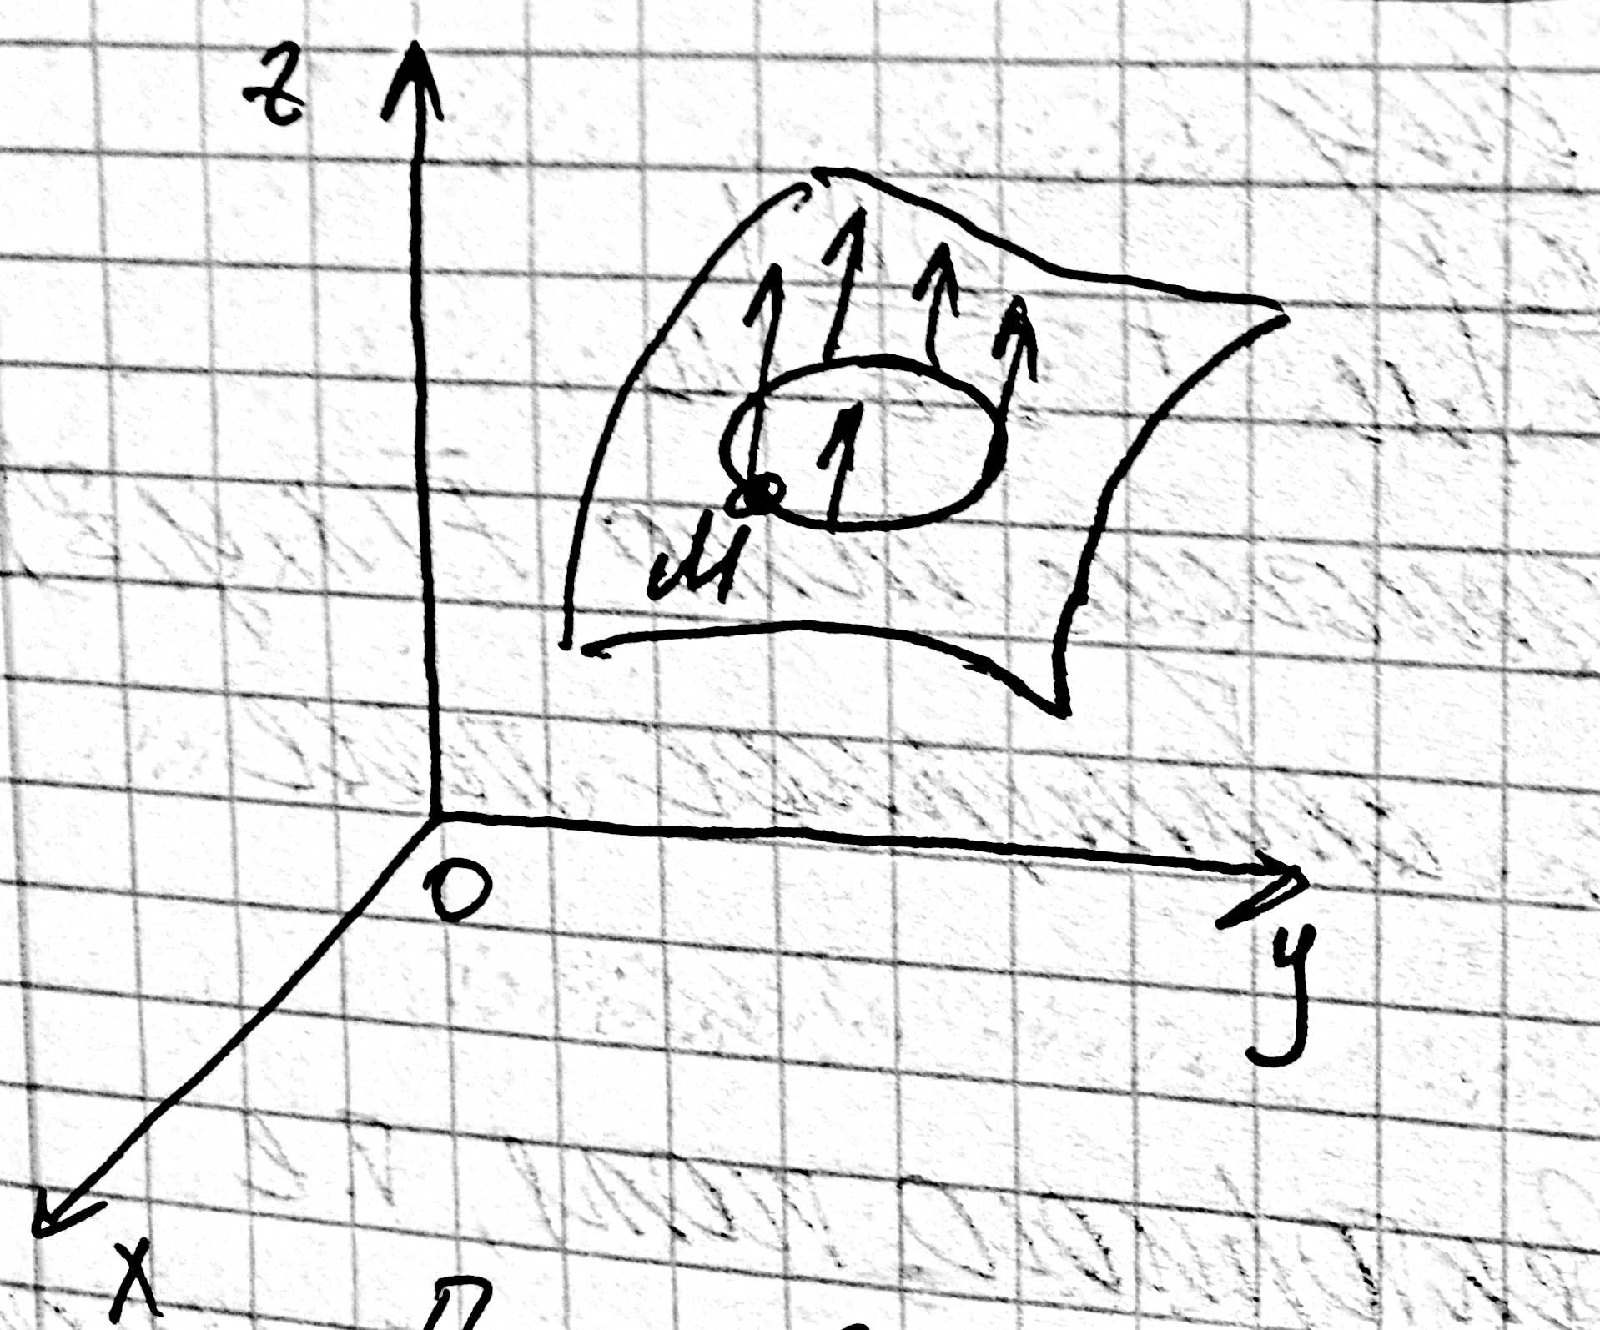
\includegraphics[width=\linewidth]{img/3.jpg}

Пусть в пространстве дана гладкая поверхность $\sigma$. На этой поверхности выберем произвольную точку $M$ и проведем через нее вектор нормали $\overrightarrow{n}$ к поверхности. Через точку $M$ на поверхности $\sigma$ так же проведем произвольный контур, не имеющий общих точек с границей поверхности $\sigma$.

Точку $M$ вместе с вектором нормали будем перемещать по контуру так, чтобы вектор нормали постоянно был перпендикулярен поверхности $\sigma$. 

По возвращении точки $M$ в начальное положение возможны 2 случая: направление $\overrightarrow{n}$ сохранится или поменяется на противоположное. 

Если направление $\overrightarrow{n}$ не поменяется, то поверхность $\sigma$ называется \textbf{двусторонней}.

Если же при обходе контура контура направление $\overrightarrow{n}$ изменится на противоположное, то $\sigma$ - \textbf{односторонняя} 

Двусторонние поверхности называются ориентированными, а односторонние - неориентированными.

Для односторонней поверхности не вводится понятие интеграла 2 рода

\subsection{Понятие площади поверхности}

Пусть $G$ - гладкая (кусочно-гладкая) ограниченная поверхность. Разобьем ее гладкими кривым произвольно на $n$ частей так, чтобы каждая из этих площадок однозначно проецировалась на касательную плоскость, проведенную  в любой точке элементарной площадки.

На каждой элементарной площадке $G_i$ выберем произвольную точку $M_i$ и проведем через эти точки касательные плоскости к поверхности. 

Обозначим через $S_i$ площадь проекции $G_i$ на свою касательную плоскость (эта поверхность ограничена кусочно-гладкими кривыми и потому квадрируема)

Составим сумму: $S(G_i,M_i) = \sum\limits_{i=1}^{n}S_i$\\
Пусть $d_i$ - диаметр $G_i$, $d= d_i (i= 1,2,..,n)$

Если существует предел $\lim\limits_{n\to\infty, d\to 0} S_n = S$, то поверхность называется квадрируемой, а число $S$ - ее площадью